\externaldocument{Files/PersonasGroup}
\subsection{Structure}
\label{ApplicationStructure}
In this section we will describe how the prototype for the project has been realized, starting with and introduction to the technologies and services used, a description of the goals the app aims to achieve and details such as the structure of the database. Technical details of the implementation have been intentionally left out of this report given that it's not meant to be a design document or a how-to guide on how the application was built, since that would need a lengthy and appropriate document by itself. Instead, the aim of the following sections is to explain what the application does and the logic/reasoning behind the main choices that have been made during its development such as which services have been implemented and how data is handled.
\subsection{Introduction}
\label{App:Introduction}
\subsubsection{Operating System: Android}
Given previous experience with it, we decided to build the prototype on Android (with minimum sdk 23 and compiled on skd 28), since the popular open source operative system is free to develop on by anyone without needing any particular machine or license (unlike for example iOS), and is instead sufficient to use Android Studio\footnote{\url{https://developer.android.com/studio/}} that comes also with the proper emulator software for testing purposes without the need to connect a physical device (which is still possible to do by simply installing the USB drivers).
\subsubsection{Development Platform: Firebase}
\label{sub:Firebase}
Firebase\footnote{\url{https://firebase.google.com/}} is Google's platform to develop web and mobile applications, which offers a number of services free to use on a small scale (but more than enough for our project purposes). Specifically we took advantage of:
\begin{itemize}
\item Authentication: handles in a standard way the registration and login of the users by allowing them to access with different methods by using a normal email address and password or connecting via popular verified systems such as Gmail, Facebook, Twitter and others, assigning them a UID to each identity.
\item Database: as we will discuss more in detail in \autoref{App:DatabaseStructure} we used both database systems:
	\begin{itemize}
	\item Realtime database: fast and reliable, worse web interface and poor query 	capability as it doesn't allow chaining commands.
	\item Cloud Firestore: just released from beta, it has an easier to read web interface and it allows more powerful queries with 			chaining and indexing.
	\end{itemize}
\item Storage: since neither of the database systems allow to store files but only Objects (strings, numbers, maps, arrays, etc...) a storage system has been used to store the users' profile images.
\item Cloud Functions: used to perform server side actions when a given trigger is fired, a more in depth description can be found in \autoref{App:CloudFunctions}.
\item Cloud Messaging: used together the cloud function \emph{SendNotification} (\autoref{Sec:SendNotification}) it was used to send users notifications for new reservations and incoming chat messages.
\end{itemize}
\clearpage
\subsection{Goals}
We wanted to build a single tool for the entire target group (\autoref{TargetGroup}) and after some considerations we came up with the following goals for our platform:
\begin{itemize}
\item Allow locals to create a profile to offer fishing services with working hours.
\item Allow customers to create a profile with basic information to make reservations.
\item Allow local fishermen to be found by customers that need fishing lessons.
\item Allow locals to be found by customers that need fishing equipment.
\item Allow local expert fishermen to add fishing spots to a public list.
\item Allow customers to search for fishing lessons, renting equipment and fishing spots in the Elk River area.
\item Allow customers to contact the employees using a simple chat system and vice versa.
\item Allow customers to leave a review for any service offered.
\end{itemize}
\subsection{Database Structure}
\label{App:DatabaseStructure}
As said in \autoref{sub:Firebase} Firebase was used among other things to store data.\\
Contrary to what it's commonly used, Firebase doesn't offer a relational database and it's instead a NoSQL JSON system, where the use of duplicate data is actually encouraged by the creators to avoid a higher number of reads in order to search for the related entry.\\
What follows is the representation of the online database structure of both the \textit{Cloud Firestore} and the \textit{Realtime} (used only for storing chats) by using some examples to fill the fields and definitions instead of some of those that are not meant to be read by humans, such as UIDs (Unique Identifiers) or URLs. \\\\
Chats \autoref{Par:Chat} are stored in a different way, in the Cloud Firestore database the main collection \emph{chats} contains for each user that started at least one chat a document with that user UID, inside of this document a structure Map-like is present where the key is the \textit{other} user with whom the chat is started and the value is an object with the necessary data, meaning that for each chat two different entries are made in the Cloud Firestore database. \\
In other words if Kevin Smith starts a chat with Bob Simmons there will be two structures as follows:
\begin{itemize}
\item chats -> Kevin Smith's UID -> Bob Simmons' UID -> data
\item chats -> Bob Simmons' UID -> Kevin Smith's UID -> data
\end{itemize}
This is done because each user needs to access all their conversations when opening the chat homepage, and retrieving a single document (using their UID) is much faster than doing a query and filtering it.\\
The single conversations are instead stored in the Realtime database, where each one can be found by their UID created as \textit{smallUID\_bigUID} (where the comparison of the two is simply the result of the \textit{Java String.compareTo} method) and each message is stored under that with an auto-generated UID as key while as values only the message text and the sending user name are saved.\\
Notifications (\autoref{Par:Notification}) are stored only temporarily, once the Cloud Function \textit{sendNotification} (\autoref{Sec:SendNotification}) is triggered and it sends the notification, the entry is deleted from the database.\\
Further comments needed are written besides each field in \textcolor{ForestGreen}{green colour}.\\

\lstset{
    string=[s]{"}{"},
    stringstyle=\color{blue},
    comment=[l]{:},
    commentstyle=\color{black},
escapeinside={\\*}{*\\},    
}
\paragraph*{Customer}:
\begin{lstlisting}
{
  "uid": "Firebase generated ID",
  "name": "Kevin",
  "surname": "Smith",
  "phone": "3343200266",
  "mail": "kevin.smith@gmail.com",
  "profilePicUrl": "URL to Firebase storage" \*\textcolor{ForestGreen}{File storage is a different service}*\\
}
\end{lstlisting}
\paragraph*{Fishing Spot}:
\begin{lstlisting}
{
 "uid": "Firebase generated ID",
  "name": "Spot Fly Fishing",
  "nameLowercase": "spot fly fishing",
  "latitude": 38.53497378591452,
  "longitude": -81.71645309776068,
  "averageReviews": 0,
  "numReviews": 0
}
\end{lstlisting}
\paragraph*{Reservation}:
\begin{lstlisting}
{
  "time": "2019-08-10 17:00:00 UTC+2",
  "type": "expert_instructor",
  "employeeUid": "UID of employee reserved", \*\textcolor{ForestGreen}{null if spot reservation}*\\ 
  "spotUid": "UID of spot reserved", \*\textcolor{ForestGreen}{null if employee reservation}*\\
  "customerUid": "UID of customer reserving",
  "customerName": "Kevin Smith",
  "customerPic": "URL profile pic customer",
  "employeePic": "URL profile pic employee"  \*\textcolor{ForestGreen}{null if spot reservation}*\\
}
\end{lstlisting}
\paragraph*{Chat}: \textcolor{ForestGreen}{From Bob Simmons' database part}
\label{Par:Chat}
\begin{lstlisting}
{
  "thisName": "Bob Simmons",
  "otherName": "Kevin Smith",
  "otherUid": "Kevin Smith's UID",
  "lastText": "See you there!",
  "otherProfilePic": "Kevin Smith's profile pic URL",
  "isRead": true,
  "lastMsgDate": "2019-08-10 13:11:17 UTC+2"
}
\end{lstlisting}
\clearpage
\paragraph*{Employee}:
\begin{lstlisting}
{
  "uid": "Firebase generated ID",
  "name": "Bob Simmons",
  "mail": "bob.simmons@gmail.com",
  "address1": "Daniel St",
  "address2": "51",
  "city": "Webster Springs WV",
  "zip": "26288",
  "phone": "332655953",
  "averageReviews": 5,
  "numReviews": 1,
  "profilePicUrl": "URL to Firebase storage", \*\textcolor{ForestGreen}{File storage is a different service}*\\
  "tags": [ \*\textcolor{ForestGreen}{ArrayList<String>}*\\
    "expert_instructor"
  ],
  "hours": [ \*\textcolor{ForestGreen}{Map<String, List<String>>}*\\
    {
      "Monday": [
        "Closed",
        "Closed",
        "13:00",
        "20:00"
      ],
      "Tuesday": [
        "Closed",
        "Closed",
        "13:00",
        "20:00"
      ],
      "Wednesday": [
        "Closed",
        "Closed",
        "13:00",
        "20:00"
      ],
      "Thursday": [
        "Closed",
        "Closed",
        "13:00",
        "20:00"
      ]\*\textcolor{ForestGreen}{Cut for page length purposes}*\\
    }
  ]
}
\end{lstlisting}
\clearpage
\paragraph*{Review}:
\begin{lstlisting}
{
  "reviewScore": 4,
  "serviceUid": "UID of employee/spot",
  "customerUid": "UID customer making the review",
  "type": "review type" \*\textcolor{ForestGreen}{spot, rental or expert\_instructor}*\\
}
\end{lstlisting}
\paragraph*{Notification}:
\label{Par:Notification}
\begin{lstlisting}
\*\textcolor{ForestGreen}{Title and Body depend on the type (new reservation or chat message), but there is no need to store it.}*\\
{
  "recipientUid": "UID receiving user",
  "title": "notification title", 
  "body": "notification message"
}
\end{lstlisting}
\subsection{Cloud Functions}
\label{App:CloudFunctions}
Written in JavaScript (NodeJs) When the specified trigger is fired server side actions can be executed in order to relieve the clients from doing numerous actions that would slow down their device.
\subsubsection{New Review}
\label{Sec:NewReview}
Every time a new review is added to the database, it takes the given score and going into the employee entry it computes back the total score by multiplication between the average and the number of reviews, then it adds the new score and increments by one the total and the new average is computed and stored.\\
If the new score is a modification of an older review, then the average is updated instead by subtracting the old score from the sum before adding the new one and the total number of reviews is not incremented.
\subsubsection{Send Notification}
\label{Sec:SendNotification}
When a new notification is stored in the database it takes sends the content to all the users subscribed to the topic specified, since the topic is the UID of a user and each one is subscribed to its UID topic after the login process, only one user will receive the notification.
\clearpage
\subsection{User Interface}
\begin{samepage}
In this section the main UI screens are shown, note that the chat screen has the same interface for both kinds of users.
\subsubsection{Customer UI}
\begin{figure}[h]
\centering
\begin{subfigure}{.5\textwidth}
  \centering
  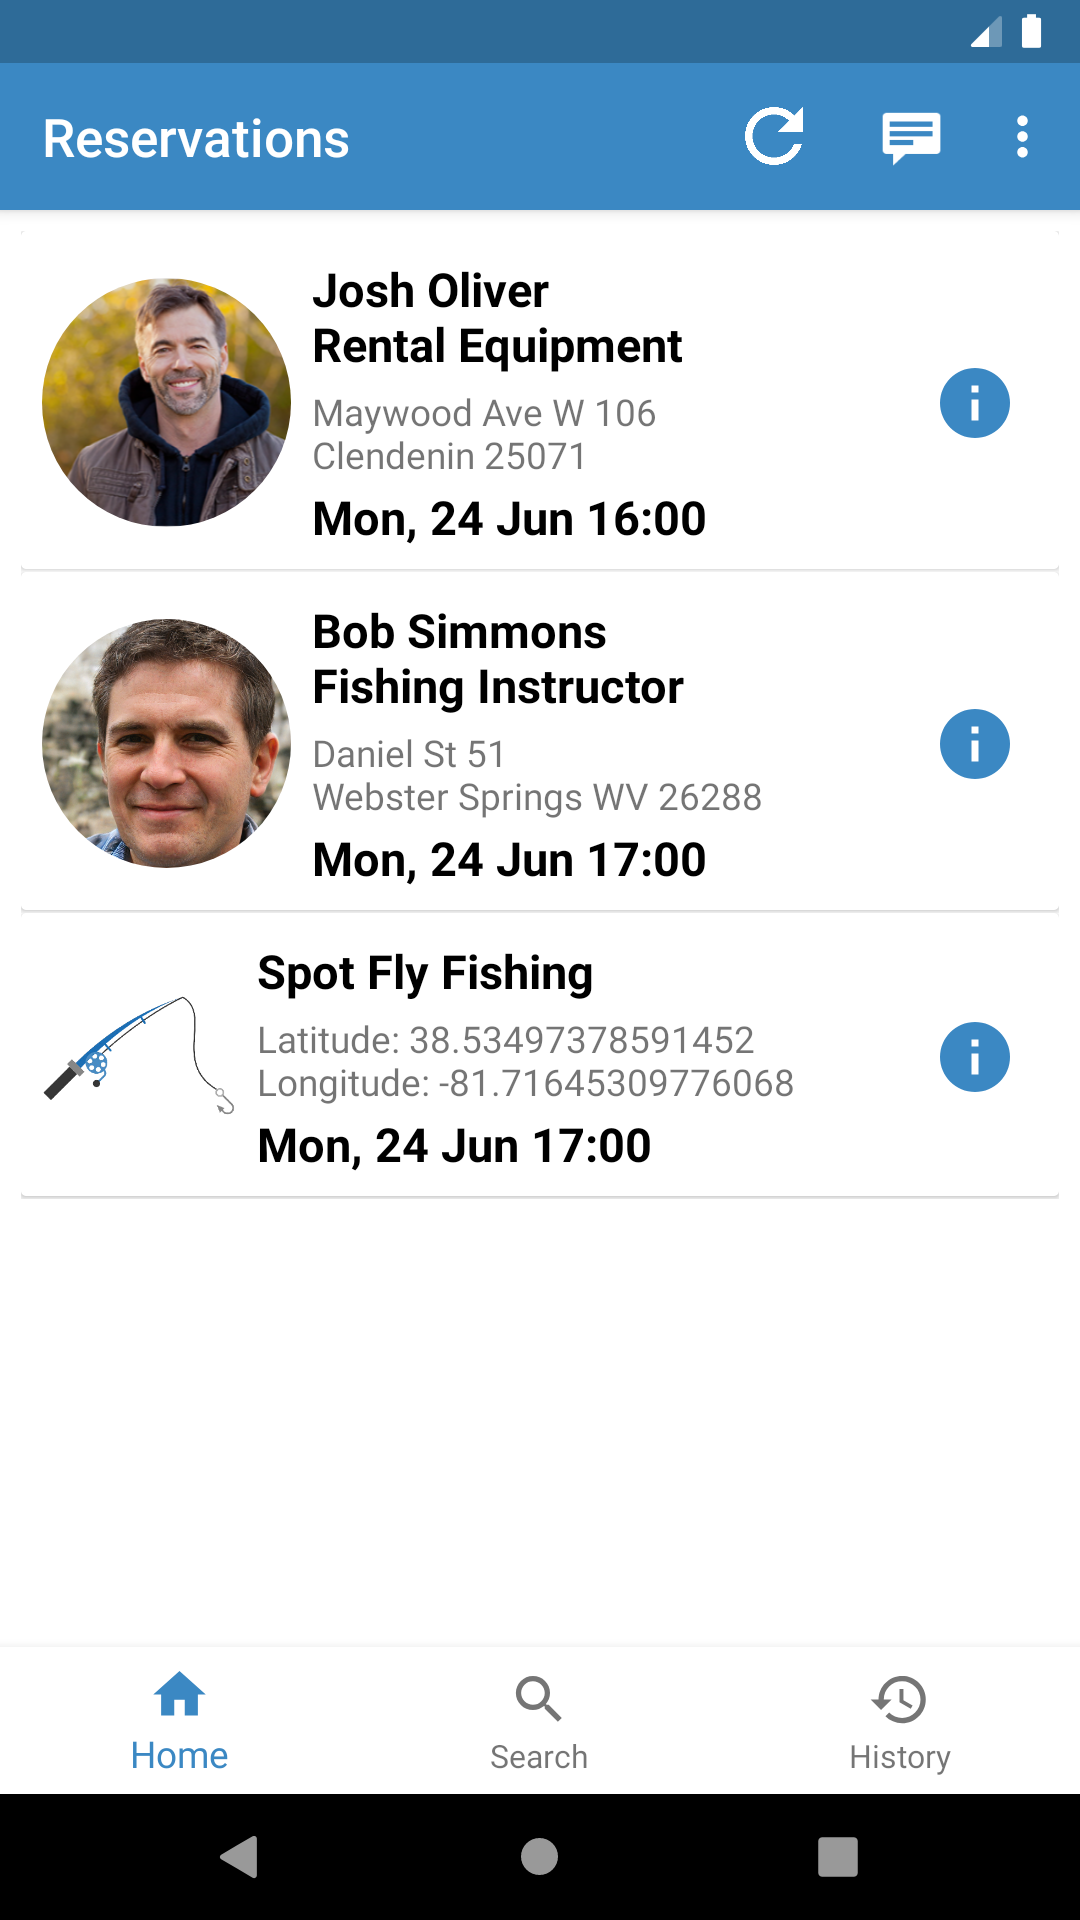
\includegraphics[height=.3\textheight, keepaspectratio=true]{Img/CustomerHome}
  \caption{Customer Homepage}
\end{subfigure}%
\begin{subfigure}{.5\textwidth}
  \centering
  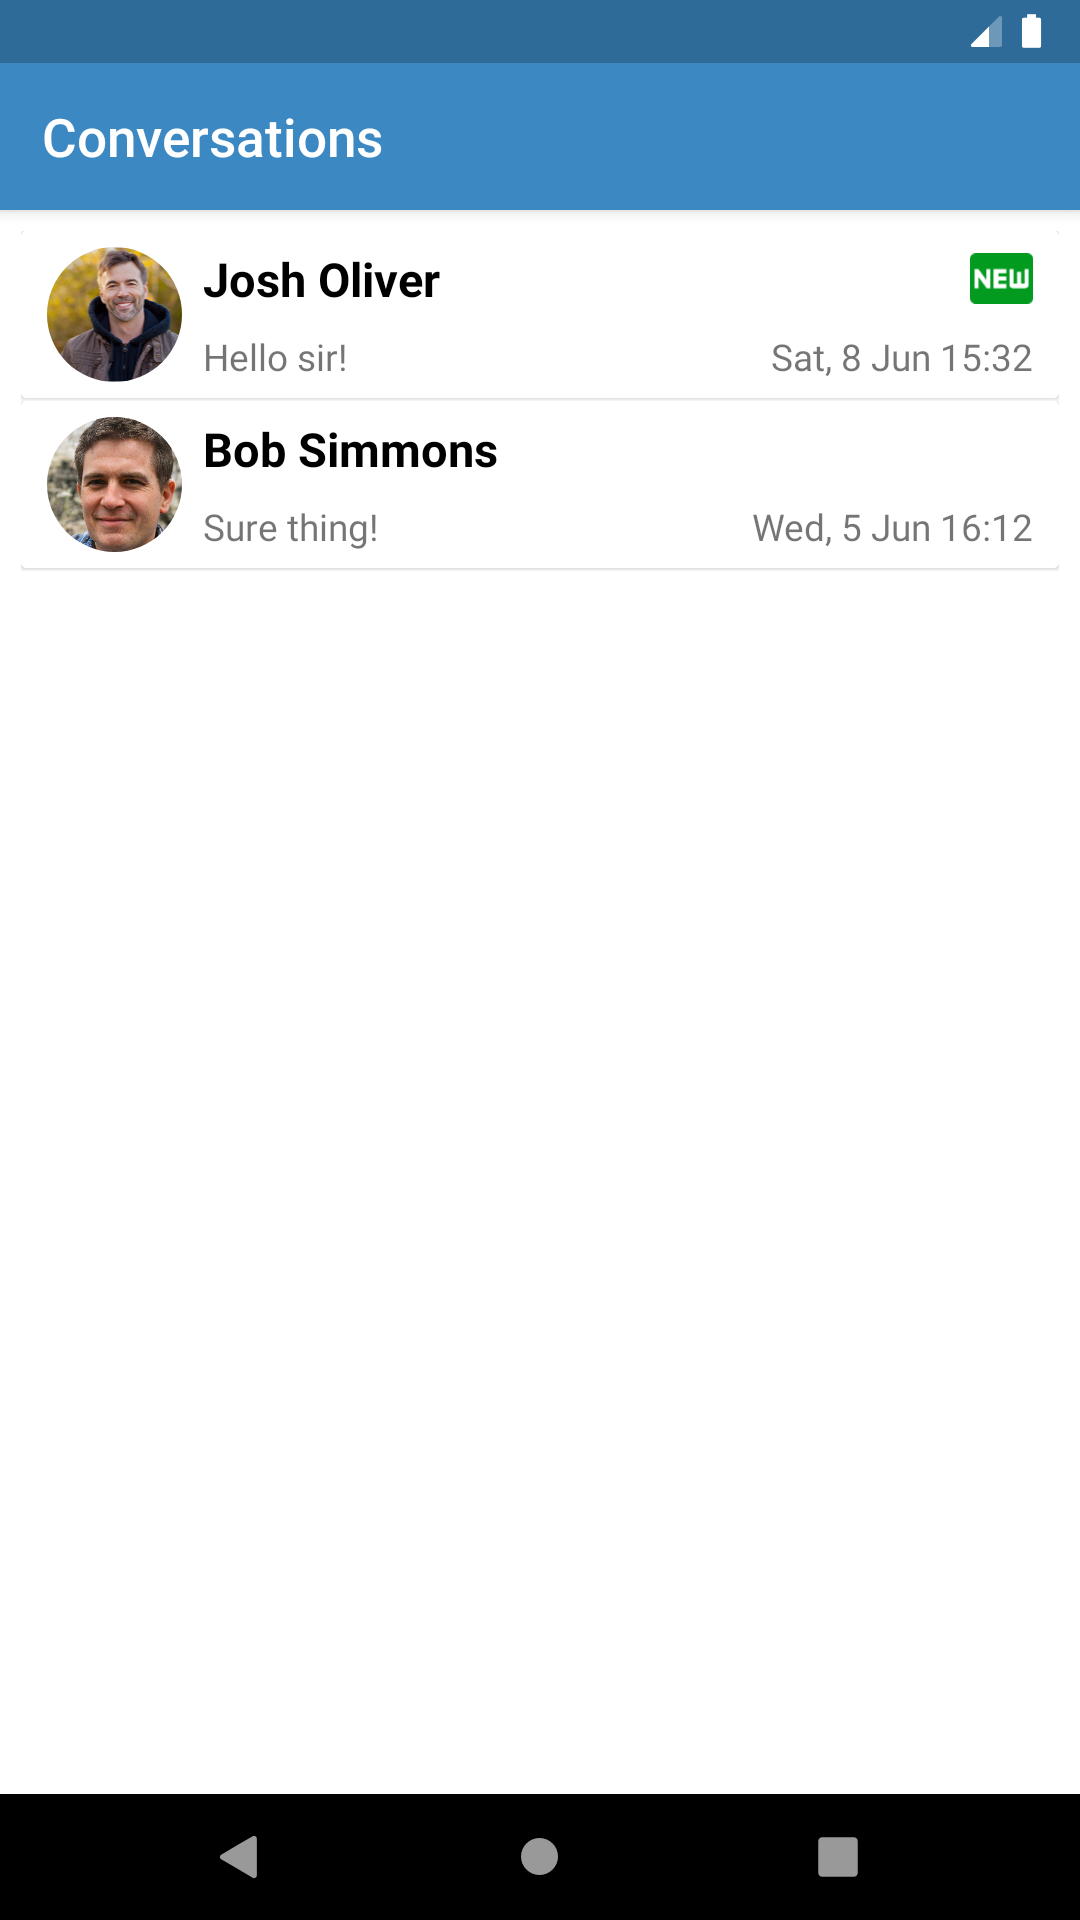
\includegraphics[height=.3\textheight, keepaspectratio=true]{Img/Chat}
  \caption{Chat main page}
\end{subfigure}
\vspace{0.5cm}
\begin{subfigure}{.5\textwidth}
  \centering
  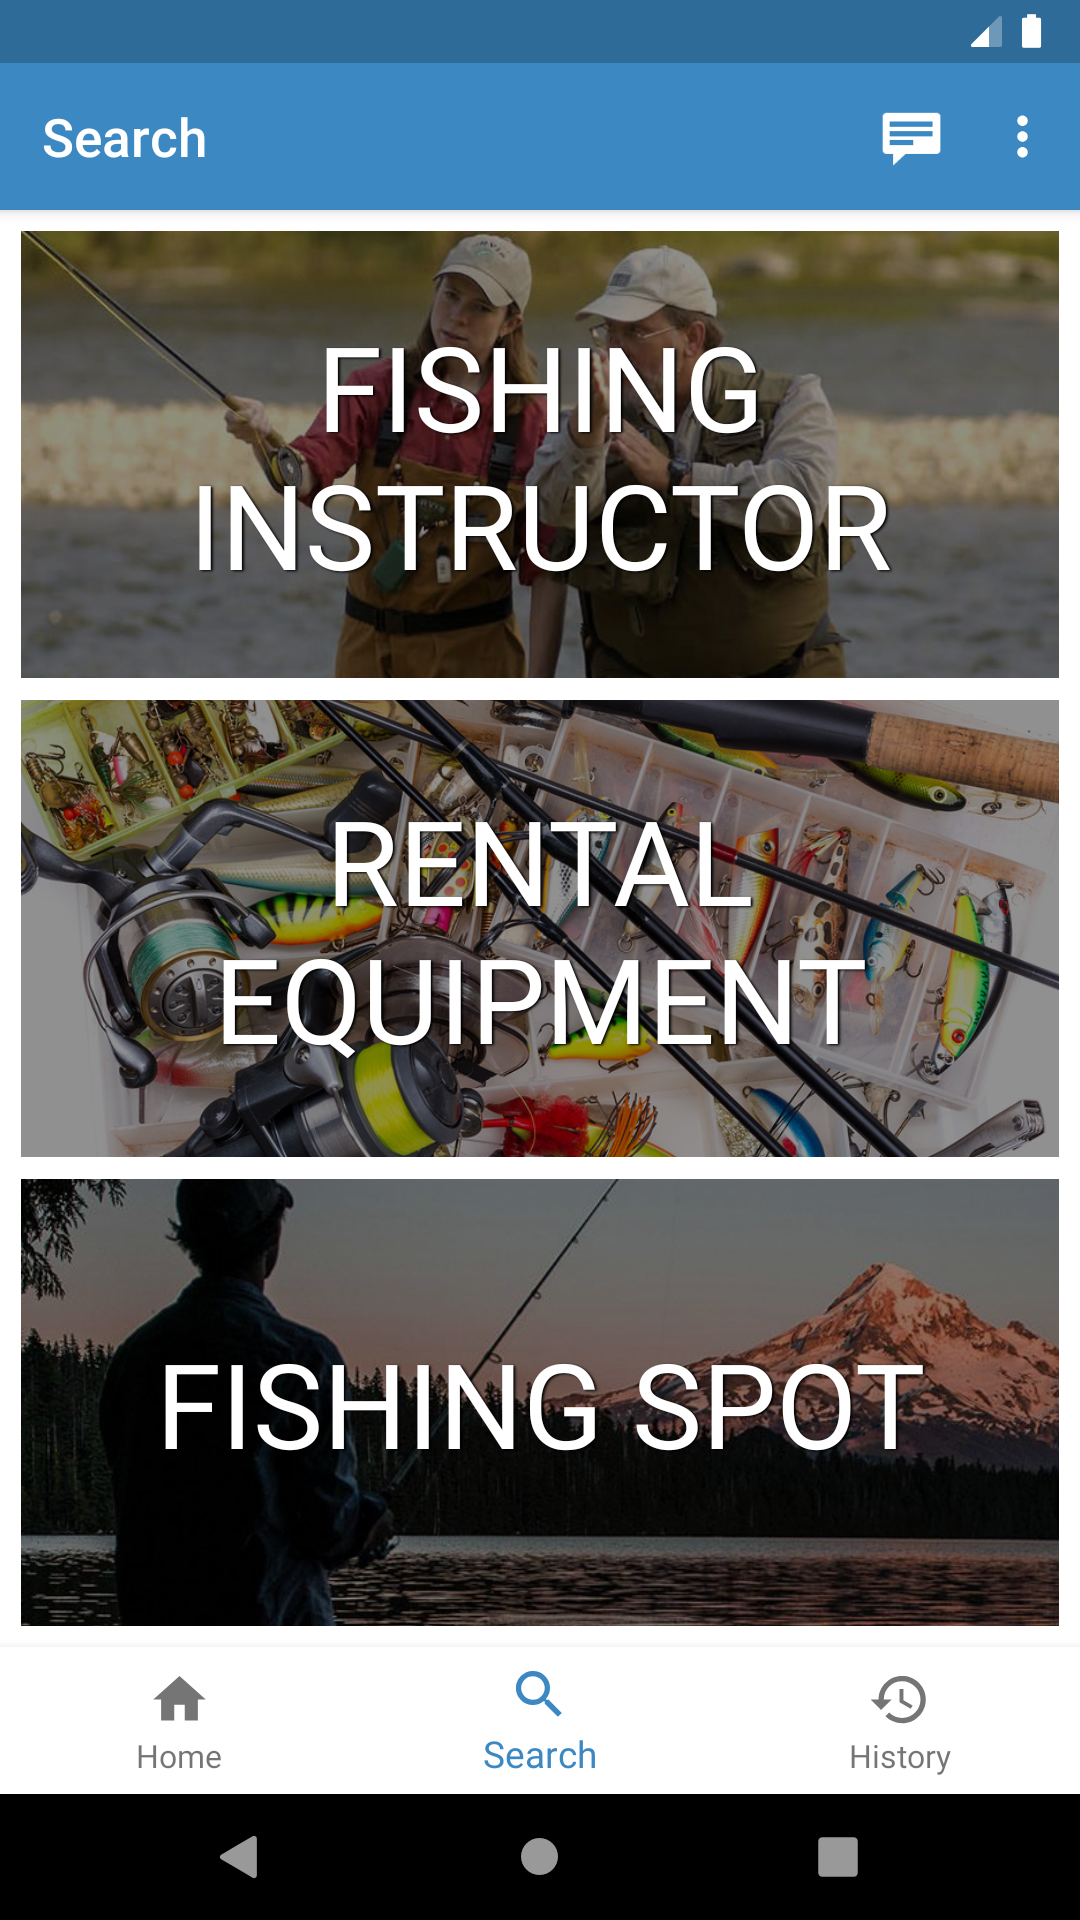
\includegraphics[height=.3\textheight, keepaspectratio=true]{Img/CustomerSearch}
  \caption{Customer main search page}
\end{subfigure}%
\begin{subfigure}{.5\textwidth}
  \centering
  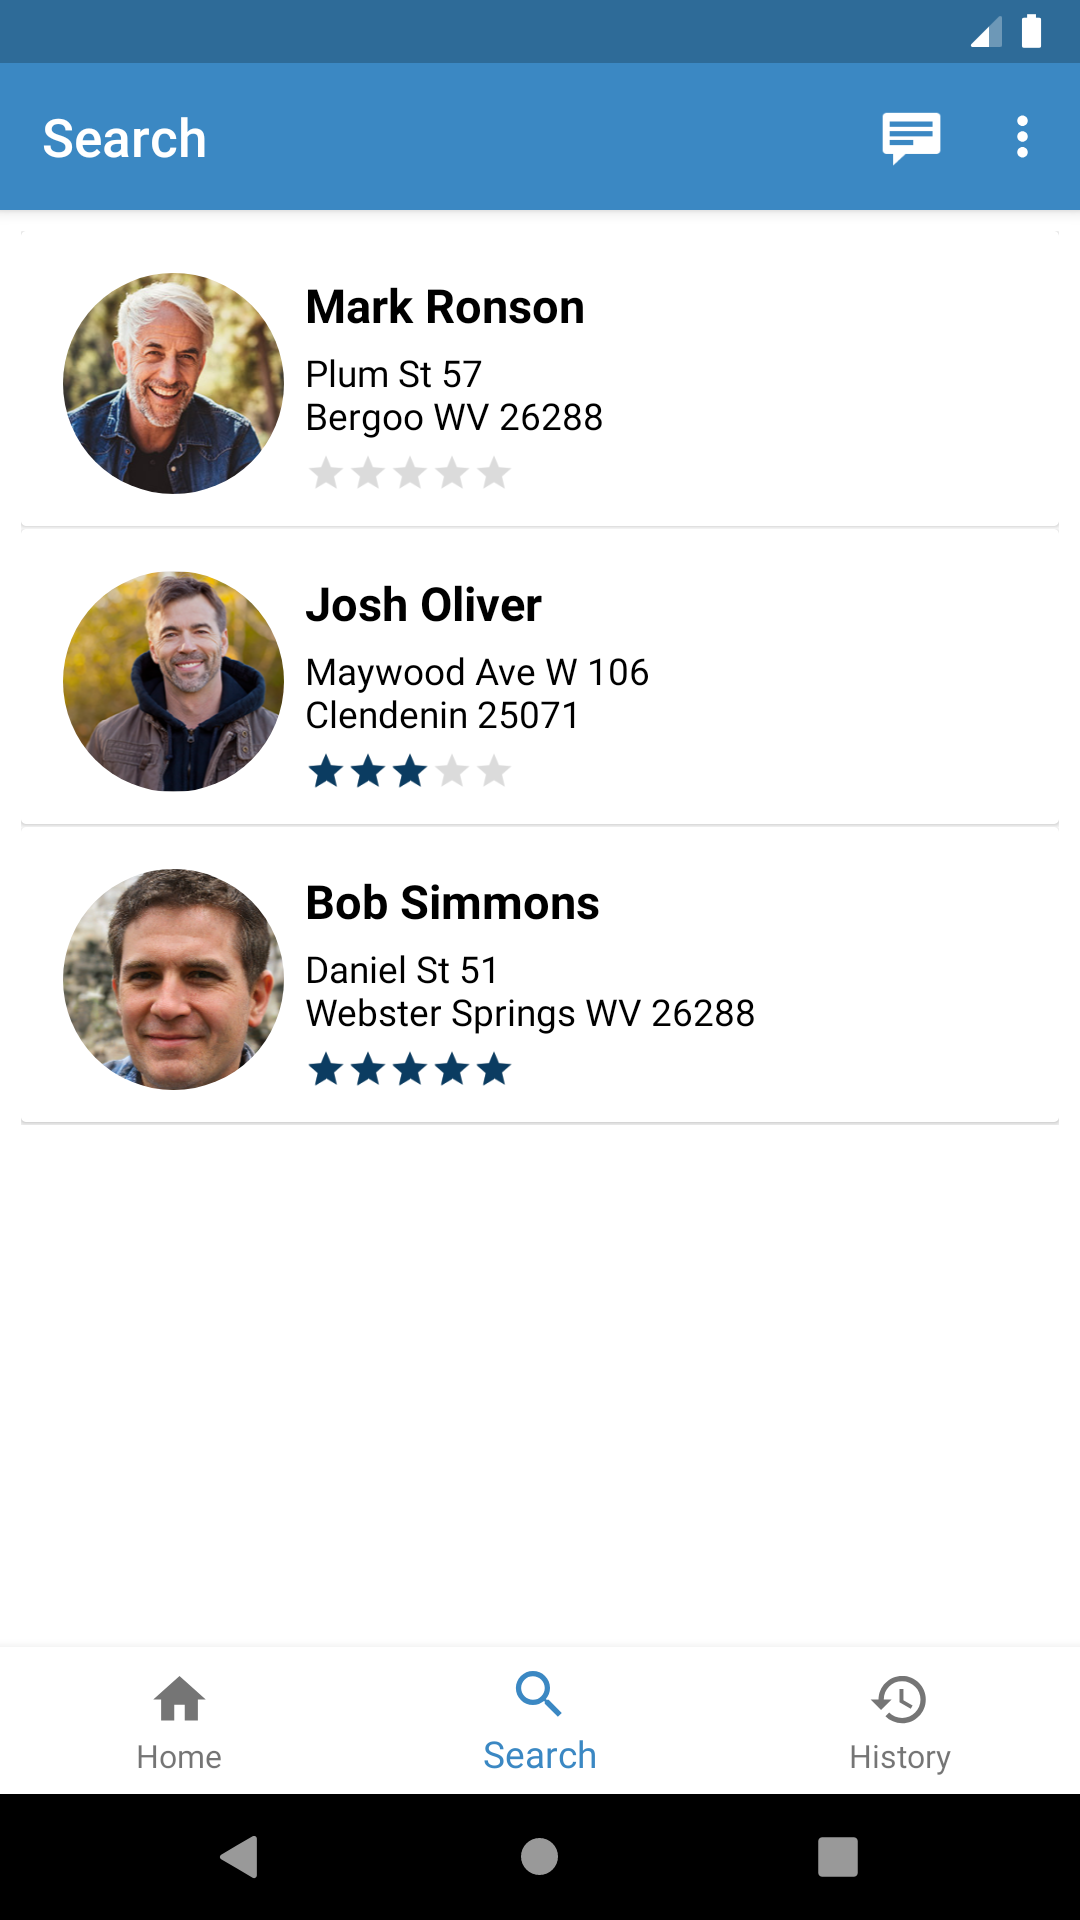
\includegraphics[height=.3\textheight, keepaspectratio=true]{Img/CustomerSearch2}
  \caption{Result of searching an instructor}
\end{subfigure}
  \caption{Customer Homepage (a), search pages (c)(d) and chat mainpage (b)}
\end{figure}
\end{samepage}
\clearpage
\subsubsection{Employee UI}
It should be noted that in \autoref{Fig:EmployeeSpot} the employee will have the option of dragging on the map (which displays all the already registered spots) to move the center cursor which will update the latitude and longitude values in real time, or he/she will be able to manually insert the values in the text-boxes, using then the "check on map" button to put the map in the specified position (only if the values correspond to a valid coordinates, otherwise an error will be shown asking the user to insert correct values). The name of the fishing spot \textbf{must} be unique to avoid confusion to the customers and since Firesbase doesn't allow queries where a string parameters ignores upper and lower cases differences as shown in \autoref{App:DatabaseStructure} fishing spots also store the name in lowercase. If no name is inserted or it's already in use an error is displayed to the user asking for a new one.
\begin{figure}[h]
\centering
\begin{subfigure}{.5\textwidth}
  \centering
  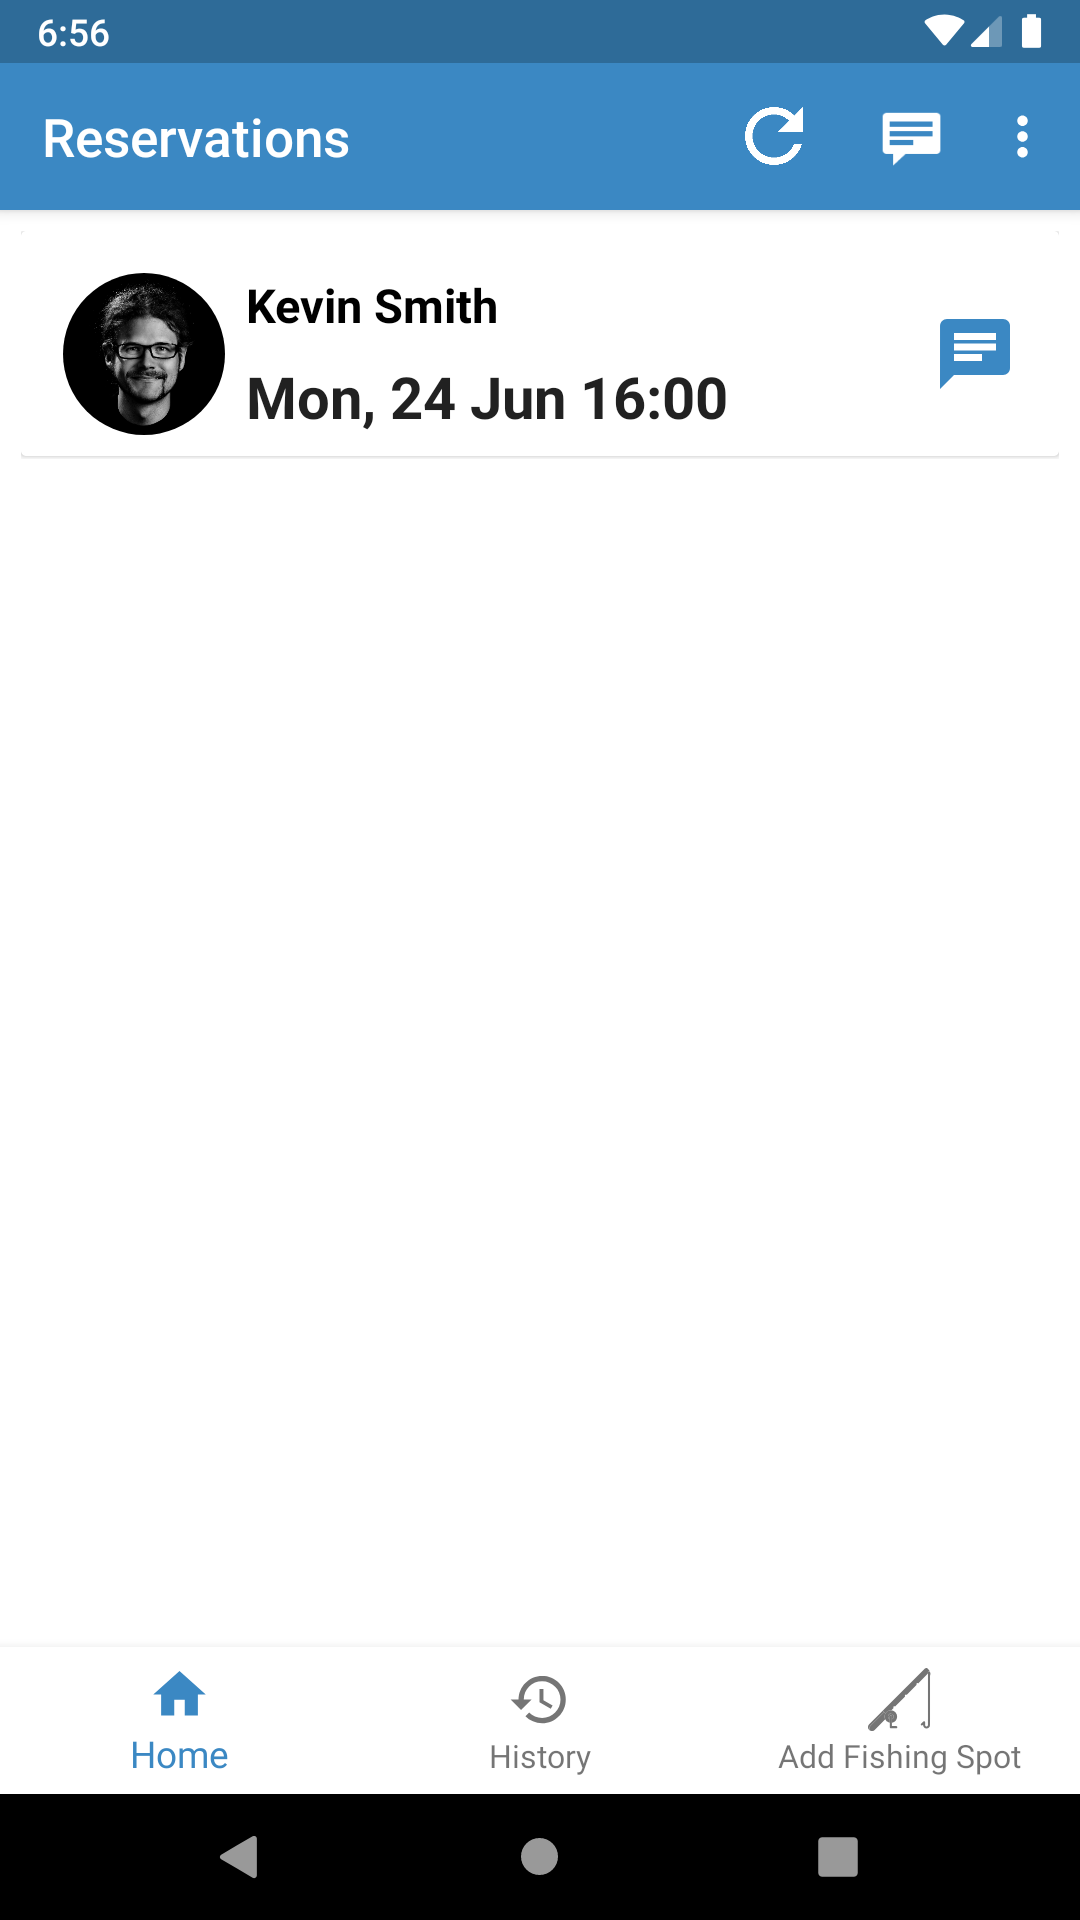
\includegraphics[height=.5\textheight, keepaspectratio=true]{Img/EmployeeHome}
  \caption{Employee Homepage}
\end{subfigure}%
\begin{subfigure}{.5\textwidth}
  \centering
  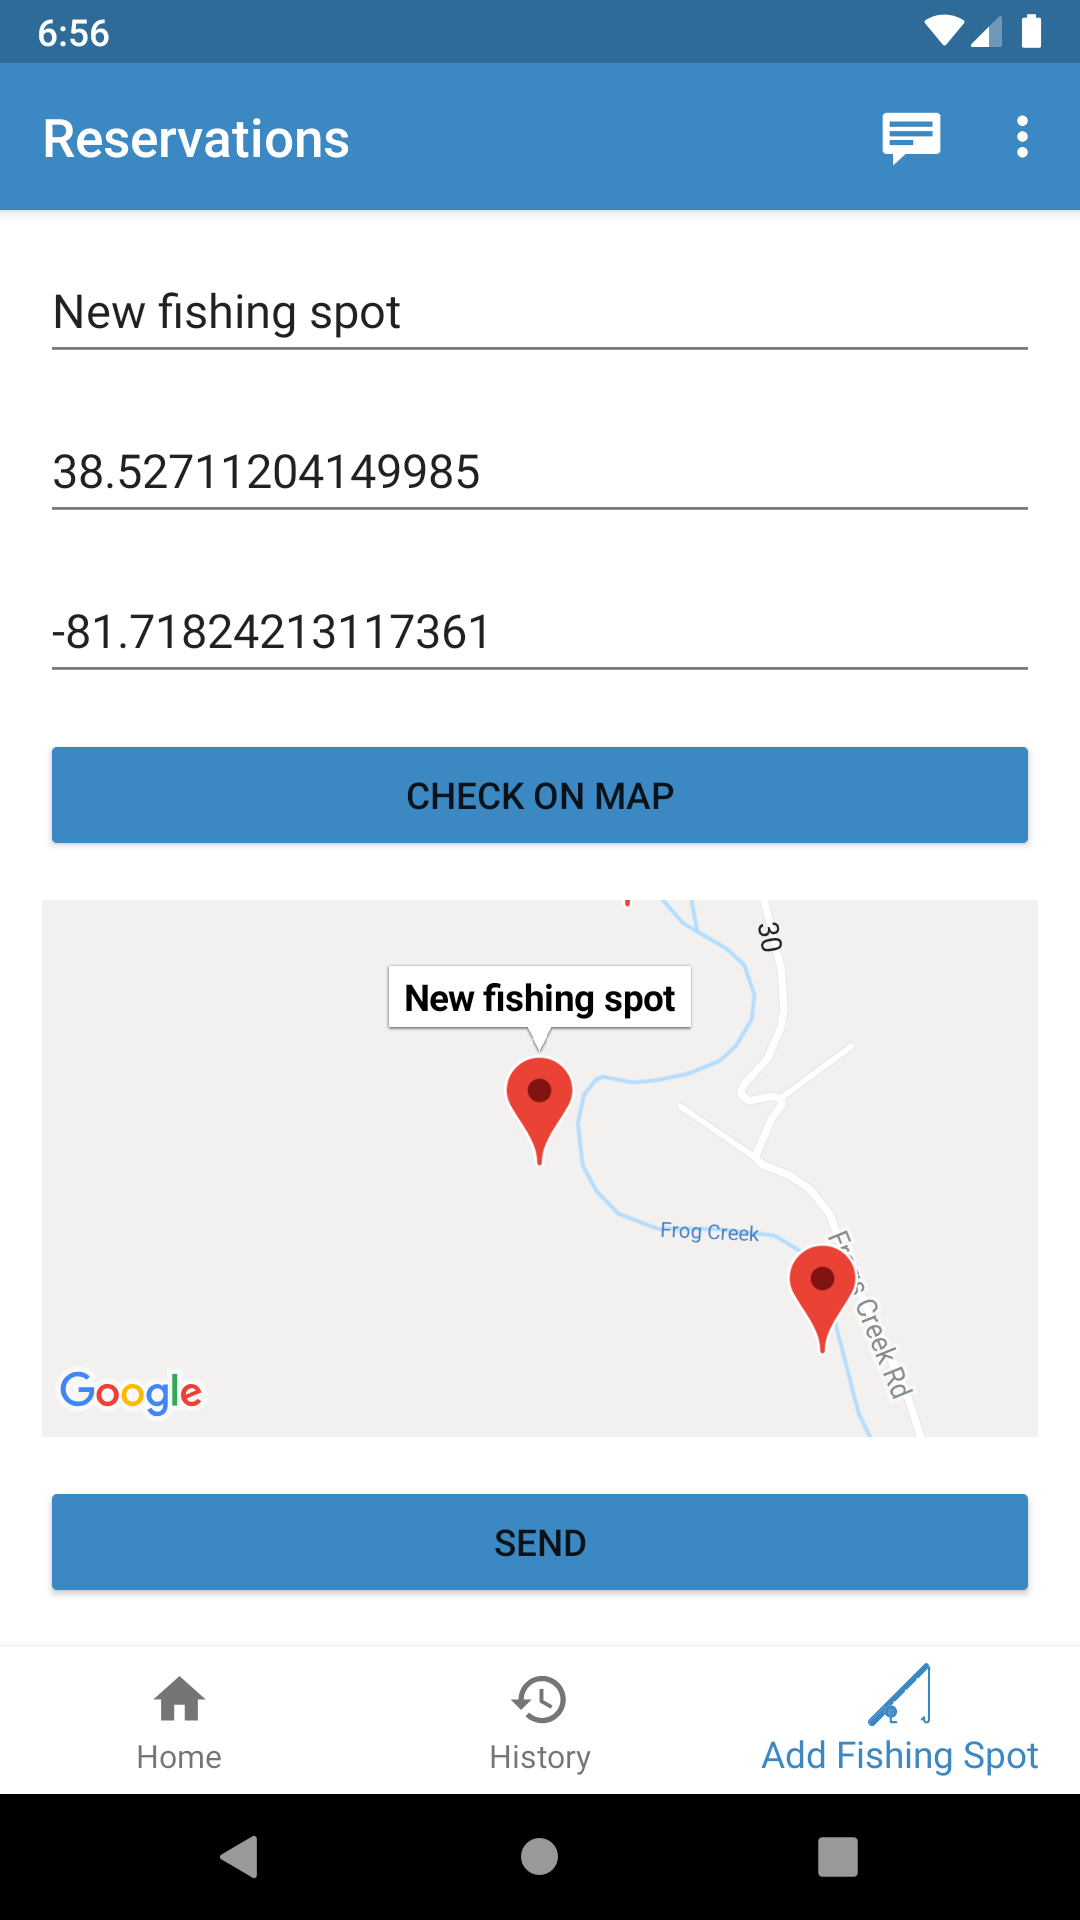
\includegraphics[height=.5\textheight, keepaspectratio=true]{Img/EmployeeSpot}
  \caption{Adding a fishing spot}
  \label{Fig:EmployeeSpot}
\end{subfigure}
  \caption{Employee Homepage (a) and new fishing spot insertion page (b)}
\end{figure}
